\documentclass[12pt]{standalone}

\usepackage{tikz}

\tikzset{
    dot/.pic = {\fill circle (2pt);}
}

\tikzset{table header/.style = {draw=none}}

\begin{document}
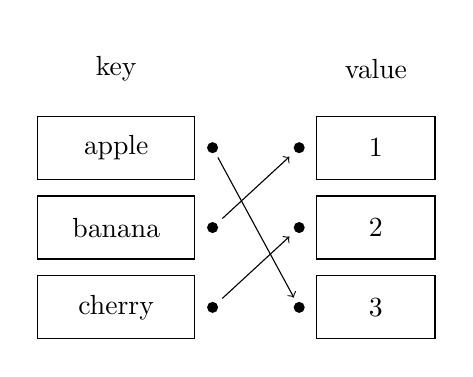
\begin{tikzpicture}

\matrix[
    row sep = 2mm,
    column sep = 1mm,
    column 1/.style = {every node/.style={draw},minimum width=20mm,minimum height=8mm},
    column 4/.style = {every node/.style={draw},minimum width=15mm,minimum height=8mm}]
{
    \node [table header] {key}; &
        &[1cm,between origins]
        &
        \node [table header] {value}; \\
    \node {apple}; & 
        \node (A) {} pic {dot}; &
        \node (1) {} pic {dot}; &
        \node {1}; \\
    \node {banana}; &
        \node (B) {} pic {dot}; &
        \node (2) {} pic {dot}; &
        \node {2}; \\
    \node {cherry}; &
        \node (C) {} pic {dot}; &
        \node (3) {} pic {dot}; &
        \node {3}; \\
};

\draw[->] (A) -- (3);
\draw[->] (B) -- (1);
\draw[->] (C) -- (2);

\end{tikzpicture}
\end{document}
